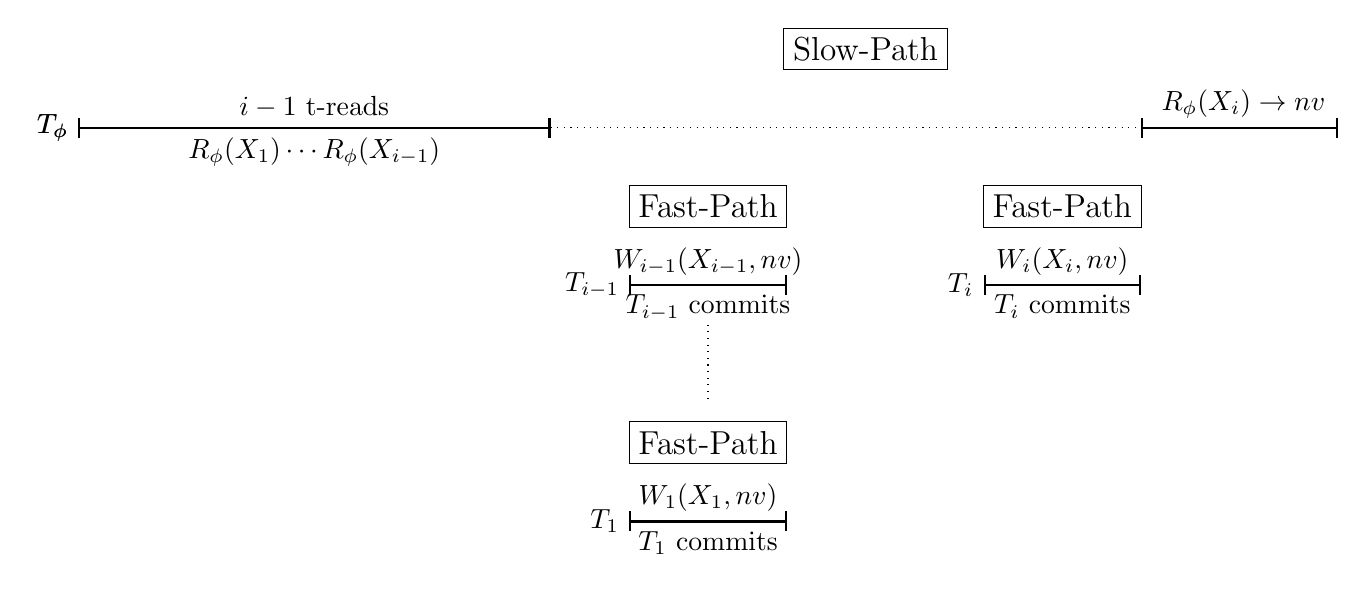
\begin{tikzpicture}
\node (r1) at (3,0) [] {};
%\node (r2) at (7.7,0) [] {};
\node (r3) at (14.8,0) [] {};


\node (w2) at (12.5,-2) [] {};
\node (w3) at (8,-2) [] {};
\node (w4) at (8,-5) [] {};


\draw (r1) node [below] {\normalsize {$R_{\phi}(X_1) \cdots R_{\phi}(X_{i-1})$}};
\draw (r1) node [above] {\normalsize {$i-1$ t-reads}};

\draw (w2) node [above] {\normalsize {$W_{i}(X_{i},nv)$}}; 
\draw (w2) node [below] {\normalsize {$T_{i}$ commits}};

\draw (w3) node [above] {\normalsize {$W_{i-1}(X_{i-1},nv)$}}; 
\draw (w3) node [below] {\normalsize {$T_{i-1}$ commits}};

\draw (w4) node [above] {\normalsize {$W_{1}(X_{1},nv)$}}; 
\draw (w4) node [below] {\normalsize {$T_{1}$ commits}};

\draw (r3) node [above] {\normalsize {$R_{\phi}(X_{i})\rightarrow nv$}};
\node[draw,align=left] at (10,1) {{\large Slow-Path}};
\node[draw,align=left] at (12.5,-1) {{\large Fast-Path}};
\node[draw,align=left] at (8,-1) {{\large Fast-Path}};
\node[draw,align=left] at (8,-4) {{\large Fast-Path}};
\begin{scope}   
\draw [|-|,thick] (0,0) node[left] {$T_{\phi}$} to (6,0);
\draw [|-|,dotted] (0,0) node[left] {$T_{\phi}$} to (16,0);
\draw [|-|,thick] (13.5,0) node[left] {} to (16,0);
\end{scope}
%
%
\begin{scope}   
\draw [|-|,thick] (7,-2) node[left] {$T_{i-1}$} to (9,-2);
\draw [|-|,thick] (11.5,-2) node[left] {$T_i$} to (13.5,-2);
\draw [-,dotted] (8,-2.5)  to (8,-3.5);
\draw [|-|,thick] (7,-5) node[left] {$T_1$} to (9,-5);

\end{scope}
%
\end{tikzpicture}
%